\documentclass[10pt]{scrartcl}
\usepackage[section]{placeins} 
\usepackage{float}
\usepackage{caption}
\usepackage{graphicx}
\usepackage{wrapfig} 
\usepackage{multirow}
\usepackage{xcolor}
\usepackage{hyperref}
\usepackage{listings}

\definecolor{codegreen}{rgb}{0,0.6,0}
\definecolor{codegray}{rgb}{0.5,0.5,0.5}
\definecolor{codepurple}{rgb}{0.58,0,0.82}
\definecolor{backcolour}{rgb}{0.95,0.95,0.92}

\lstdefinestyle{mystyle}{
    backgroundcolor=\color{backcolour},   
    commentstyle=\color{codegreen},
    keywordstyle=\color{magenta},
    numberstyle=\tiny\color{codegray},
    stringstyle=\color{codepurple},
    basicstyle=\ttfamily\footnotesize,
    breakatwhitespace=false,         
    breaklines=true,                 
    captionpos=b,                    
    keepspaces=true,                 
    numbers=left,                    
    numbersep=5pt,                  
    showspaces=false,                
    showstringspaces=false,
    showtabs=false,                  
    tabsize=2
}

\lstset{style=mystyle}

\usepackage[framemethod=tikz]{mdframed}
\usepackage{lipsum}
\usepackage[allowmove]{url}

\newmdtheoremenv[
  hidealllines=true,
  leftline=true,
  innerbottommargin=6pt,
  linewidth=5pt,
  linecolor=blue!40,
  leftmargin=10pt,
  innertopmargin=0pt,
  innerbottommargin=0pt,
  innerrightmargin=0pt,
]{example}{Example}

\begin{document}
\title{Framework for Systematic Comparison of Hashing-based vs. Retrieval-based methods for Cross-modal Retrieval}
% \subtitle{Subtitle}
\author{Shivangi Bithel, Dwijesh Gohil, Prabhat Kanaujia}
\maketitle

\listoffigures
% \newpage
\section{Introduction}
We live in a multi-modal world, where we can express ourselves using a variety of representation formats like text, audio, images, etc. They can be used to represent different events happening around us. To search for data across these different modalities, we have cross-modal retrieval systems. Cross-modal retrieval is a natural way of information retrieval, where the input data is given in one modality or a combination of modalities, and output data can be retrieved in another or set of different modalities. For example, given textual data, “A beautiful sunny day on the beach” we can retrieve data related to this similar event in the form of an image or a video.
\begin{figure}
    \centering
    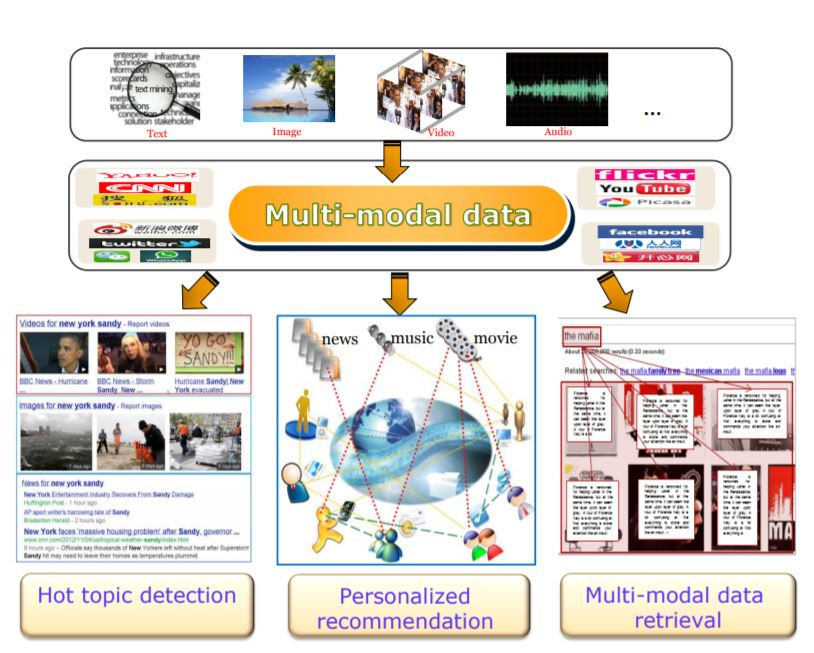
\includegraphics[width=8cm]{example1.JPG}
    \caption{Multi-modal Data}
\end{figure}
% some more points to be added in introduction
% General framework of cross-modal retrieval

% About the framework and APIs we have designed
\newpage

Major Contributions of this work are briefly summarized below: 
\begin{enumerate}
    \item We are providing a systematic framework for comparing different cross-modal retrieval algorithms.
    \item The framework evaluates two representative algorithms on the two commonly used datasets for cross-modal retrieval, namely Nuswide, XMediaNet and Wikipedia dataset.
    % \item ...about our graphs and comparison
\end{enumerate}

\section{Overview}
Cross-Modal retrieval is an important problem in real-world applications like social media. Applications like Facebook, Twitter, Instagram get thousands of GBs of new data uploaded everyday which belongs to different modalities. To solve this problem, in the literature we have two kinds of algorithms, Hashing-based retrieval algorithms and Ranking-based retrieval algorithms.
Hashing-based algorithms uses binary representation to speed up cross modal retrieval process. Data from different modalities is transformed to a common hamming  space. We then perform cross modal similarity search in this common space by comparing the hamming distance. We use binary codes to represent data, which can lead to some loss in accuracy but it is time and space efficient.
Retrieval-based ranking algorithms uses real-valued representation learning. Here, we learn a common representation space, where we can directly measure the similarity between data belonging to different modalities. These algorithms can be further categorized into supervised and unsupervised based on the methodology they use to learn the common space.
\begin{figure}
    \centering
    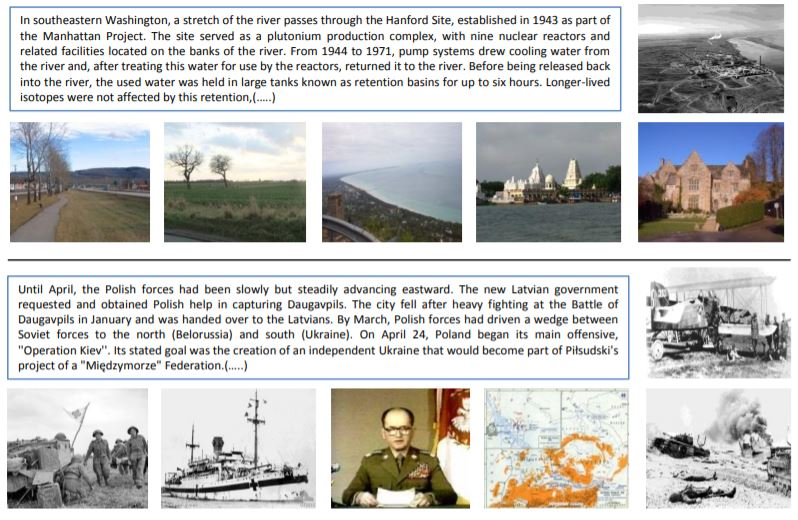
\includegraphics[width=10cm]{example2.JPG}
    \caption{Cross-modal Retrieval}
    \label{fig:example}
\end{figure}
\subsection{OCMFH}
Online Collective Matrix Factorization Hashing is an unsupervised online learning method based on collective matrix factorization hashing (CMFH). It comes as an improvement over CMFH, and provides retrieval over large-scale data in a time and space efficient manner. As we have seen in example of Instagram, social media application, which already has millions of bytes of data, and every day a large chunk of new multimedia data is added to it. In such cases, training over complete data again and again is very time and space consuming. As a solution, OCMFH uses online learning method, which updates hash functions only on the new data chunk and also generates unified hash codes. It does not refer to the "orignal old data" while adaptively updating the hash codes. OCMFH also uses a zero mean normalization to overcome the mean varying problem in online hashing methods. It takes input, Image-Text pairs, hash-code length, parameters and iteration number and provides Hash codes, image and text projection matrices and their mean vectors. For querying, it uses feature vectors, projection matrices and mean vectors as input and compute the hamming distance between the generated hash codes, which is a bitwise operation and thus it is very fast and space efficient also. 
 

\begin{figure}
    \centering
    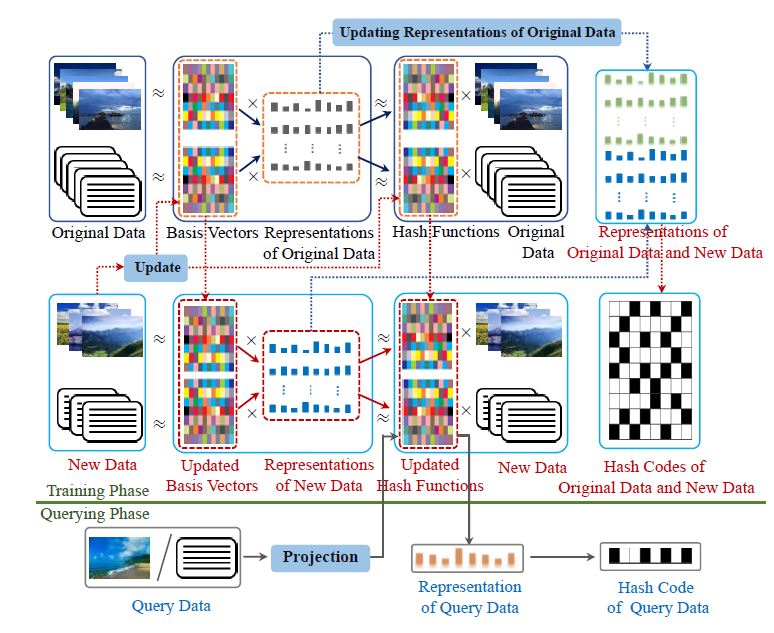
\includegraphics[width=8cm]{OCMFH.JPG}
    \caption{Framework for Online Collective Matrix Factorization Hashing}
\end{figure}


\subsection{ACMR}
Adversarial Cross-Modal Retrieval is a ranking-based retrieval algorithm, which learns a common subspace to project data from different modalites. The goal of this algorithm is to find data item projections in a common feature representation subspace. ACMR combines the concept of supervised representation learning for cross-modal retrieval and adversarial learning. For input, ACMR takes image and text features, labels, hyperparameters, and samples in minibatch for each modality, and generates learned representation in common subspace. ACMR uses two processes, first is feature projector, which generates modality-invariant representation for items from different modalities in the common subspace. Its objective is to confuse the second process, which is a modality classifier. Modality classifier tries to differentiate between modalities and thus guide the feature projector to learn better representations which are invariant to the modality. The feature projector jointly performs label prediction so that underlying cross-modal semantic structure of the data can be preserved. Thus the feature representations are both invariant across the modalities and discriminative within a modality. For querying, we project input features in one modality and query features in other modality and calculate the distance between the two features. The features with higher similarity will have minimum distance even though they belong to different modalities. 

\begin{figure}
    \centering
    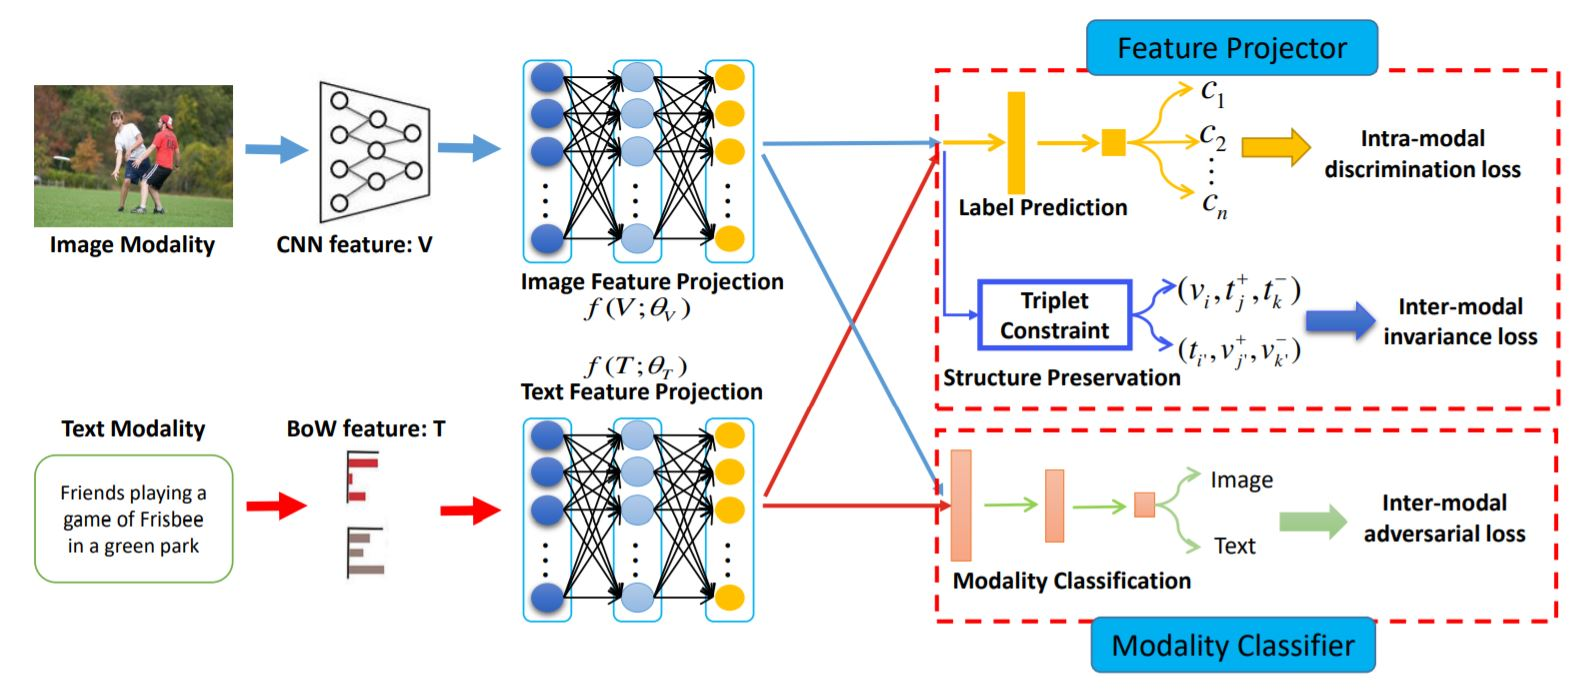
\includegraphics[width=0.8\linewidth]{ACMR.JPG}
    \caption{Flowchart of ACMR method}
    \label{fig:my_label}
\end{figure}

\section{Dataset}
\subsection{Xmedianet}
    Xmedianet dataset can be downloaded from \href{https://drive.google.com/file/d/1OYv7IK5OdDmBQ_pRXMugnqZzR_j7HOsu/view?usp=sharing}{here}. In the following experiments, we use only image and text features, though Xmedianet dataset comes with features of other modality as well(e.g. audio, video, etc.). Xmedianet dataset has 200 categories, 8000 test samples, and 32,000 train samples. We use this dataset without any pre-processing or filtering process.
\subsection{NUS-WIDE}
    NUS-WIDE dataset can be downloaded from \href{https://lms.comp.nus.edu.sg/wp-content/uploads/2019/research/nuswide/NUS-WIDE.html}{here}. It is a multi-label dataset with image and text modality features. It has 81 ground truth categories but we use top-20 most frequent categories. We exclude any sample which does not have any ground truth category assigned. After such pre-processing, it has 83,644 train samples, 4402 test samples.\\
    Another variant for the same dataset is being used in ACMR algorithm, which is NUS-WIDE 10K.
    This dataset can be downloaded from \href{https://github.com/shivangibithel/ACMR_demo/tree/master/data}{here}. It uses 8000 training samples, 2000 testing samples and one sample only has one associated label, from the available 10 labels. Image feature vectors are 4096d, extracted using FC7 layer of VGGNet. Text samples are represented using 1000d Bag-of-words representation.   
\subsection{Wiki}
    Wikipedia dataset can be downloaded from \href{https://github.com/shivangibithel/ACMR_demo/tree/master/data/wikipedia_dataset}{here}.
    In the ACMR algorithm, we are using this wikipedia dataset, which has 1300 training image-text pairs and 1566 testing image-text pairs. These are publically available 128d SIFT features for images and 10d LDA features. Only one label out of available 10 labels are assigned to the image-text pairs. 

\section{Framework}
We provide a framework for end-to-end experiments and comparisons across models. The framework consists of 3 primary components:
\subsection{Dataset}
\begin{lstlisting}[language=Python, caption=Dataset initializer]
def __init__(self, directories,
                     loader, 
                     preprocess=None,
                     preprocess_params=None,
                     normalize=None,
                     normalization_params=None,
                     read_directories=(True,True,True),
                     summarize=None
                     ):
\end{lstlisting}
Dataset class provides a wrapper for loading, preprocessing, normalizing and summarizing train, validation and test datasets. The format for storing, preprocessing, normalizing and summarizing the dataset is user-defined, as per the corresponding functions.\\
This modular approach allows the user to change a particular aspect of the dataset, while keeping others fixed, thus allowing for effective comparisons.
\subsection{Model}
\begin{lstlisting}[language=Python, caption=Model initializer]
def __init__(self, 
            training_function,
            hyperparams,
            dataset_obj,
            params=None,
            params_verification=None,
            prediction_function=None,
            evaluation_metrics=None,
            is_neural=None
            ):
\end{lstlisting}
Model class also has a modular structure. 
\begin{itemize}
    \item The parameter - training\_function, takes as an input a function. This function is core to the model class object. It has to be provided by the user and should point to a function which performs the training procedure for the concerned model.
    \item  Hyperparams, params are user-defined objects and it is up to the user to ensure consistent-use in the training and predictions functions provided by them.
    \item dataset\_obj is an object of Dataset class, as defined above
    \item evaluation\_metrics are currently fixed and limited to Precision, Recall and MAP
\end{itemize}

This framework allows the user to change certain aspects of the model, such as hyperparameters, easily and run the experiments end-to-end. Result can be exported to a file and using the Comparator class defined later, a broad range of measures can be compared across multiple models.

An example of an experimentation routine (for OCMFH algorithm is detailed below):
\begin{lstlisting}[language=Python, caption=Model training]
dataset_filepath = '/mnt/f/mtp/dataset/dataset/xmedianet/'
#dataset_filepath = '/mnt/f/mtp/dataset/dataset/nus_wide/NUS-WIDE/'
data = Dataset((dataset_filepath, dataset_filepath, dataset_filepath), 
				loaderXmedianet, read_directories=(True, False, True), summarize=summarizeDataset)
data.load_data()
hyperparams = {'bits':64, 'lambda_':0.5, 'mu':100, 'gamma':0.001, 'iter':100, 'cmfhiter':100}
params = Parameters({'PI':None, 'PT':None, 'HH':None, 'B_Tr' : None, 'B_Ir' : None, 'B_Te' : None, 'B_Ie' : None})
model = Model(	train, 
				hyperparams, 
				data, 
				params, 
				None, #params_verification 
				predict, #prediction_function
				None, #evaluation_metrics
				False) #isneural
model.train_model()
model.predict('test')
model.evaluate(data.get_train_labels(), data.get_test_labels())
model.save_stats('ocmfh_xmedianet_stats_{}bits.npy'.format(hyperparams['bits']))
\end{lstlisting}
Stats for a particular experiment can be exported to a file, and such files can be used to compare models on various metrics. 
\subsection{Comparator}
Comparator class takes a list of filenames as an input and loads and stores the corresponding stats.
Following this, 2 kinds of plots are provided out-of-the-box:
\begin{itemize}
    \item bar plots
    \item line plots
\end{itemize}
There are some restrictions regarding the structure of the stats\_file, for these curves. Please refer to the comments and documentation for more info. Custom functions can be added on top of the comparator class, if needed, making the framework extensible. For examples of what kinds of plots one can expect, please refer to the next section.\\
Sample code is also provided along with the Comparator class, in compare.py, to demonstrate how graphs can be plotted for multiple files and statistics.

\section{Results}
    \subsection{Loss History}
    Following are the loss vs iteration graphs. First plot compares ACMR\cite{acmr} and OCMFH\cite{ocmfh} on nuswide dataset. Remaining graphs are for OCMFH\cite{ocmfh} algorithm for varying bit length on both nuswide and xmedianet dataset.
        \begin{figure}[H]
            \begin{minipage}[!h]{0.6\linewidth}
                \centering
                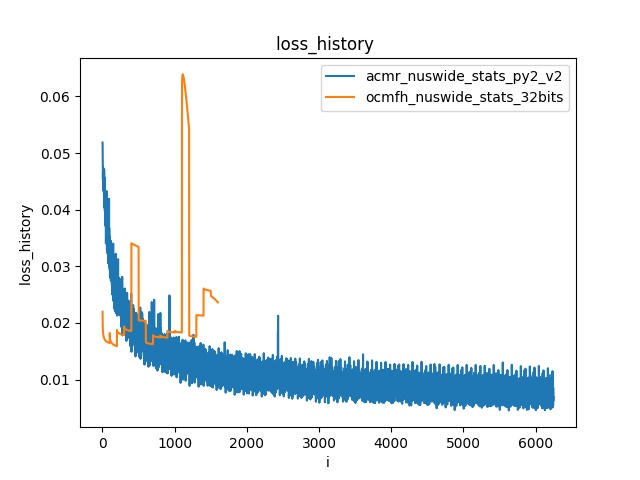
\includegraphics[width=\linewidth]{resultsImages/lossHistory/loss_history_both_nuswide.jpeg}
                % \caption{Inter comparison(NUS-WIDE)}
                % \label{fig:}
                \vspace{0.1ex}
                \hspace{0.1ex}
            \end{minipage}
            \begin{minipage}[!h]{0.6\linewidth}
                \centering
                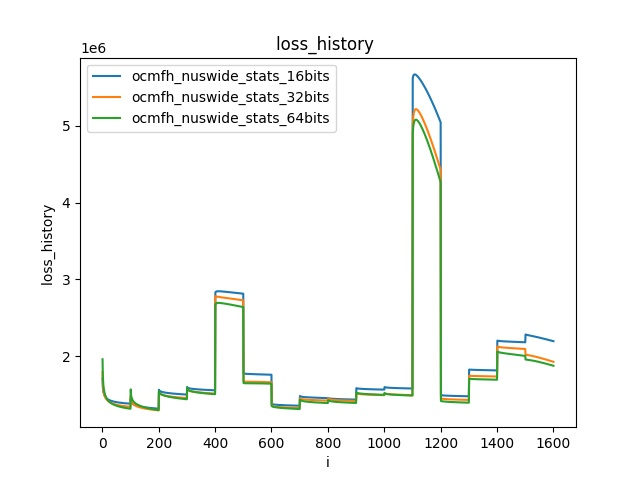
\includegraphics[width=\linewidth]{resultsImages/lossHistory/loss_history_ocmfh_nuswide_bits.jpeg}
                % \caption{OCMFH changing bits(NUS-WIDE)}
                % \label{fig:}
                \vspace{0.1ex}
                \hspace{0.1ex}
            \end{minipage}
            \begin{minipage}[!h]{0.7\linewidth}
                \centering
                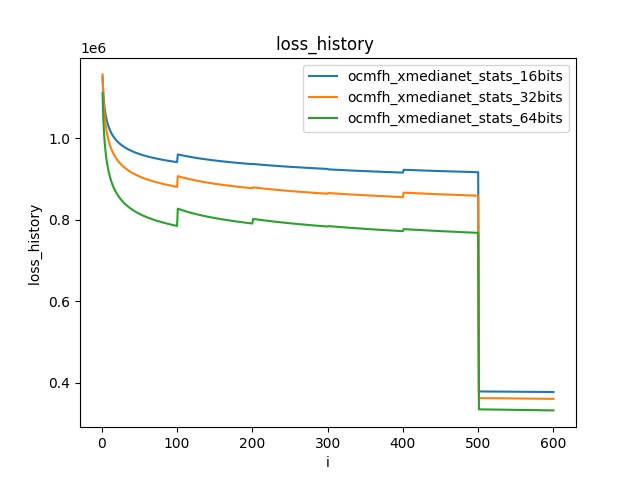
\includegraphics[width=\linewidth]{resultsImages/lossHistory/loss_history_ocmfh_xmedianet_bits.jpeg}
                % \caption{OCMFH chaning bits(Xmedianet)}
                % \label{fig:}
                \vspace{0.1ex}
                \hspace{1ex}
            \end{minipage}
            \caption{Loss vs iteration graph for inter and intra method comparison}
        \label{fig:}
        \end{figure}
        \FloatBarrier
    \subsection{Mean Average Precision}
    Following are the mean average precision vs i (mAP @ i) graph. First two graph are for OCMFH\cite{ocmfh} on nuswide dataset for varying bit length. One graph for image to text(itot) and one graph for text to image(ttoi). Remaining two graphs compares ACMR\cite{acmr} and OCMFH\cite{ocmfh} on wiki and nuswide dataset respectively for both itot and ttoi task.
        \begin{figure}[H]
            \begin{minipage}[!h]{0.6\linewidth}
                \centering
                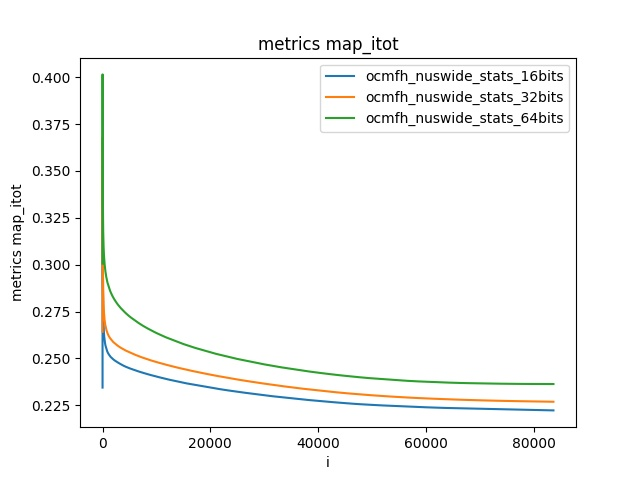
\includegraphics[width=\linewidth]{resultsImages/map/metrics map_itot_ocmfh_nuswide.jpeg}
                % \caption{Query type: min}
                % \label{fig:six_core_min}
                % \vspace{0.1ex}
                % \hspace{0ex}
            \end{minipage}
            \begin{minipage}[!h]{0.6\linewidth}
                \centering
                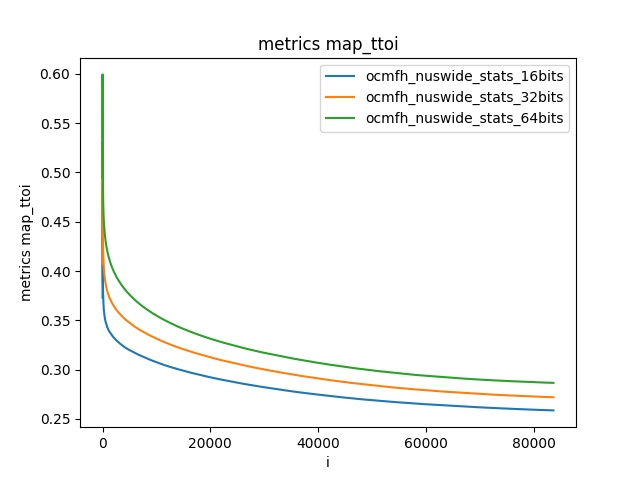
\includegraphics[width=\linewidth]{resultsImages/map/metrics map_ttoi_ocmfh_nuswide.jpeg}
                % \caption{Query type: sum}
                % \label{fig:six_core_sum}
                % \vspace{0.1ex}
                % \hspace{0ex}
            \end{minipage}
            \begin{minipage}[!h]{0.6\linewidth}
                \centering
                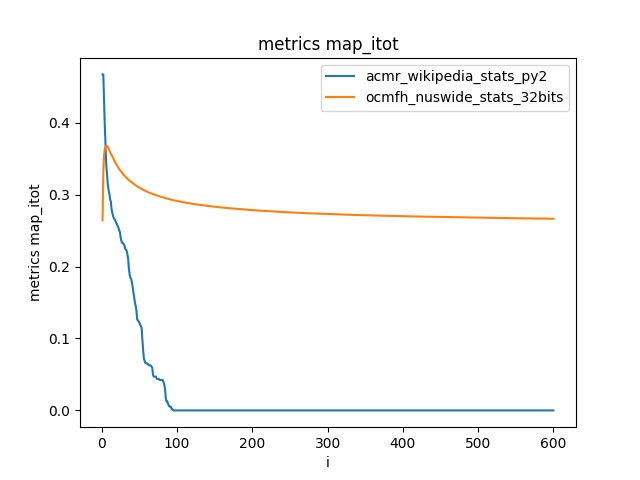
\includegraphics[width=\linewidth]{resultsImages/map/metrics map_itot_both_both.jpeg}
                % \caption{Query type: countrange}
                % \label{fig:six_core_countrange}
                % \vspace{0.1ex}
                % \hspace{0.1ex}
            \end{minipage}
            \begin{minipage}[!h]{0.6\linewidth}
                \centering
                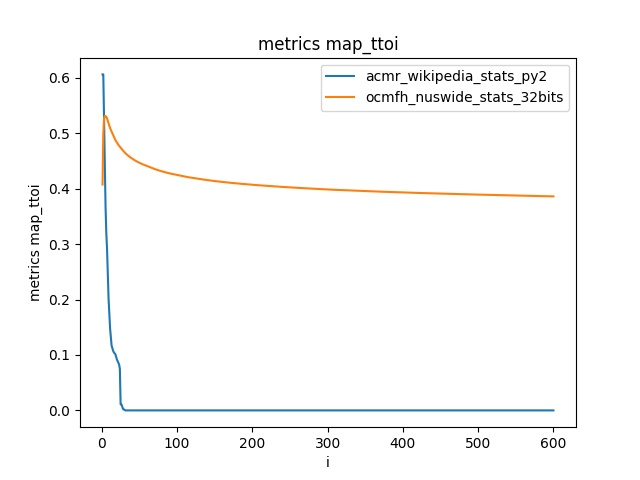
\includegraphics[width=\linewidth]{resultsImages/map/metrics map_ttoi_both_both.jpeg}
                % \caption{Query type: max}
                % \label{fig:six_core_max}
                % \vspace{0.1ex}
                % \hspace{0.1ex}
            \end{minipage}
        \caption{mAP metric for intra and inter method comparison on various datasets}
        \label{fig:}
        \end{figure}
        \FloatBarrier
    \newpage
\subsection{Precision VS Recall}
    Following are the precision vs recall curves. All of them are for OCMFH\cite{ocmfh} on both datasets(nuswide and xmedianet) for both tasks(itot and ttoi) with varying bit vector length.
        \begin{figure}[H]
            \begin{minipage}[!h]{0.6\linewidth}
                \centering
                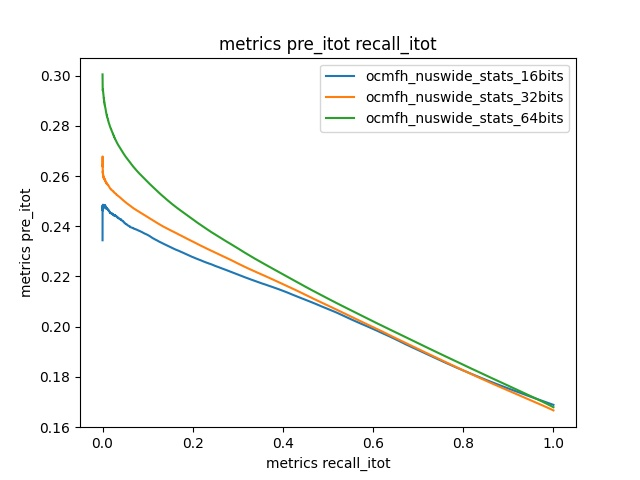
\includegraphics[width=\linewidth]{resultsImages/precisionVsRecall/metrics pre_itot recall_itot_ocmfh_nuswide.jpeg}
                % \caption{Query type: min}
                % \label{fig:six_core_min}
                % \vspace{0.1ex}
                % \hspace{0ex}
            \end{minipage}
            \begin{minipage}[!h]{0.6\linewidth}
                \centering
                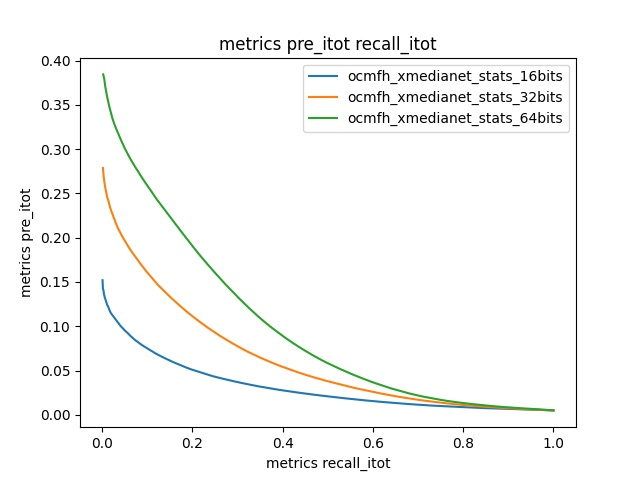
\includegraphics[width=\linewidth]{resultsImages/precisionVsRecall/metrics pre_itot recall_itot_ocmfh_xmedia.jpeg}
                % \caption{Query type: sum}
                % \label{fig:six_core_sum}
                % \vspace{0.1ex}
                % \hspace{0ex}
            \end{minipage}
            \begin{minipage}[!h]{0.6\linewidth}
                \centering
                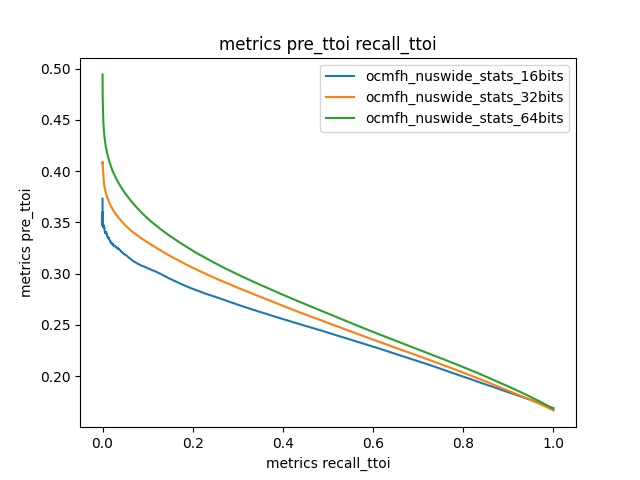
\includegraphics[width=\linewidth]{resultsImages/precisionVsRecall/metrics pre_ttoi recall_ttoi_ocmfh_nuswide.jpeg}
                % \caption{Query type: countrange}
                % \label{fig:six_core_countrange}
                % \vspace{0.1ex}
                % \hspace{0.1ex}
            \end{minipage}
            \begin{minipage}[!h]{0.6\linewidth}
                \centering
                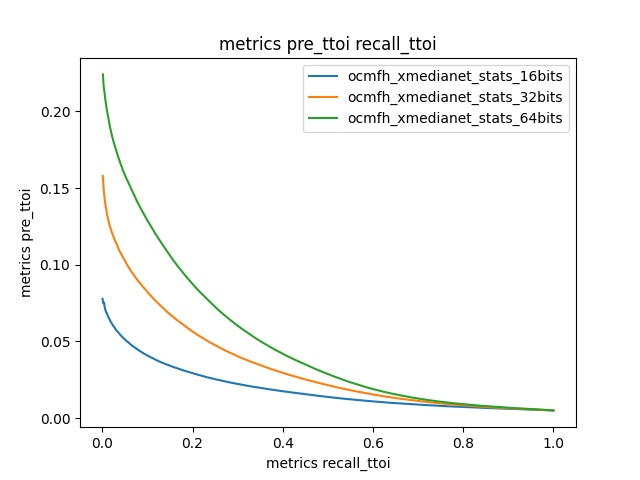
\includegraphics[width=\linewidth]{resultsImages/precisionVsRecall/metrics pre_ttoi recall_ttoi_ocmfh_xmedia.jpeg}
                % \caption{Query type: max}
                % \label{fig:six_core_max}
                % \vspace{0.1ex}
                % \hspace{0.1ex}
            \end{minipage}
        \caption{Precision vs Recall curve for OCMFH on various datasets}
        \label{fig:}
        \end{figure}
        \FloatBarrier
    \newpage
\subsection{Precision}
    Following are the precision @ i curves. Graphs in the first column are for OCMFH\cite{ocmfh} on two different datasets with fixed bit vector length(16). Graphs in the second column compares the precision value on varying bit vector length for OCMFH\cite{ocmfh} on nuswide dataset.
        \begin{figure}[H]
            \begin{minipage}[!h]{0.6\linewidth}
                \centering
                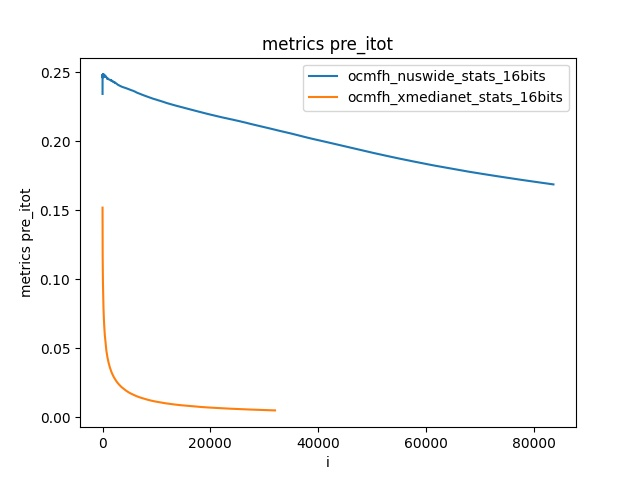
\includegraphics[width=\linewidth]{resultsImages/precision/metrics pre_itot_ocmfh_both.jpeg}
                % \caption{Query type: min}
                % \label{fig:six_core_min}
                % \vspace{0.1ex}
                % \hspace{0ex}
            \end{minipage}
            \begin{minipage}[!h]{0.6\linewidth}
                \centering
                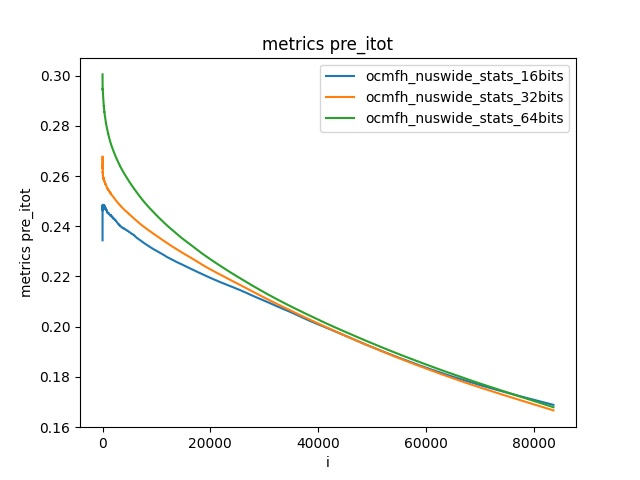
\includegraphics[width=\linewidth]{resultsImages/precision/metrics pre_itot_ocmfh_nuswide.jpeg}
                % \caption{Query type: sum}
                % \label{fig:six_core_sum}
                % \vspace{0.1ex}
                % \hspace{0ex}
            \end{minipage}
            \begin{minipage}[!h]{0.6\linewidth}
                \centering
                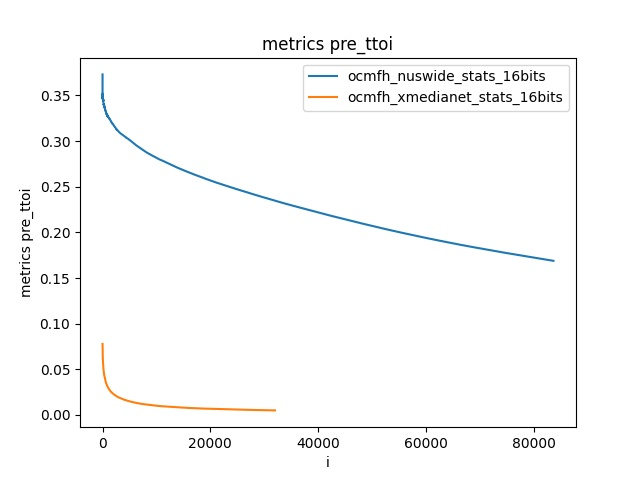
\includegraphics[width=\linewidth]{resultsImages/precision/metrics pre_ttoi_ocmfh_both.jpeg}
                % \caption{Query type: countrange}
                % \label{fig:six_core_countrange}
                % \vspace{0.1ex}
                % \hspace{0.1ex}
            \end{minipage}
            \begin{minipage}[!h]{0.6\linewidth}
                \centering
                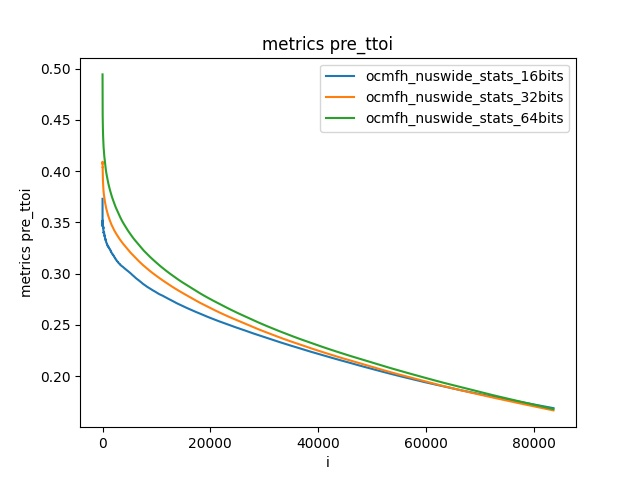
\includegraphics[width=\linewidth]{resultsImages/precision/metrics pre_ttoi_ocmfh_nuswide.jpeg}
                % \caption{Query type: max}
                % \label{fig:six_core_max}
                % \vspace{0.1ex}
                % \hspace{0.1ex}
            \end{minipage}
        \caption{Precision metric for OCMFH on various datasets}
        \label{fig:}
        \end{figure}
        \FloatBarrier
    \newpage
\subsection{Recall}
    Following are the recall @ i curves. Plots are shown for both ACMR\cite{acmr} and OCMFH\cite{ocmfh} on various datasets(nuswide, xmedianet, and wiki) with varying bit vector length.
        \begin{figure}[H]
            \begin{minipage}[!h]{0.5\linewidth}
                \centering
                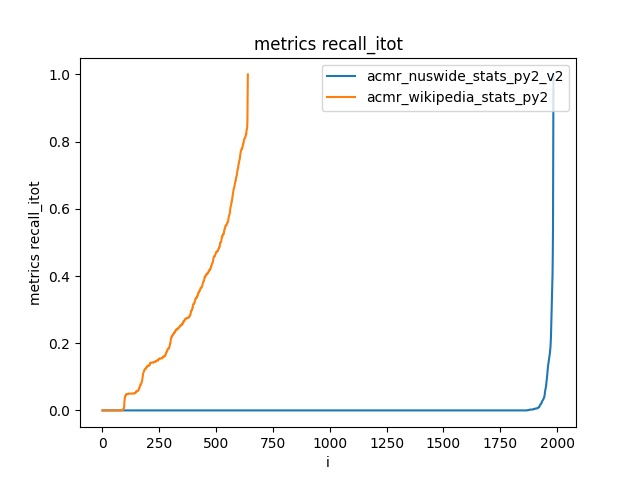
\includegraphics[width=\linewidth]{resultsImages/recall/metrics recall_itot_acmr_both.jpeg}
                % \caption{Query type: min}
                % \label{fig:six_core_min}
                % \vspace{0.1ex}
                % \hspace{0ex}
            \end{minipage}
            \begin{minipage}[!h]{0.5\linewidth}
                \centering
                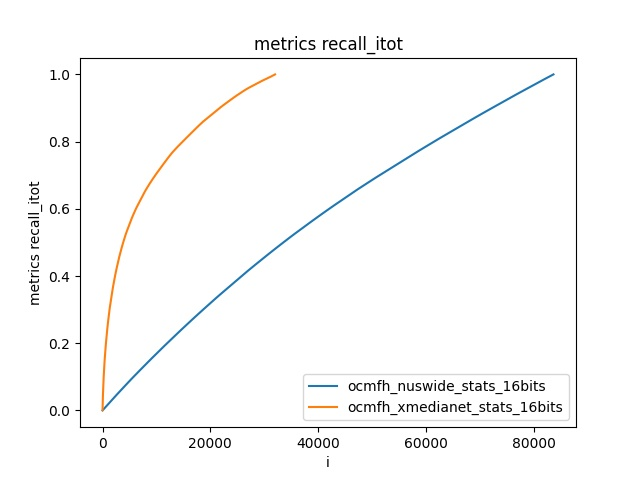
\includegraphics[width=\linewidth]{resultsImages/recall/metrics recall_itot_ocmfh_both.jpeg}
                % \caption{Query type: sum}
                % \label{fig:six_core_sum}
                % \vspace{0.1ex}
                % \hspace{0ex}
            \end{minipage}
            \begin{minipage}[!h]{0.5\linewidth}
                \centering
                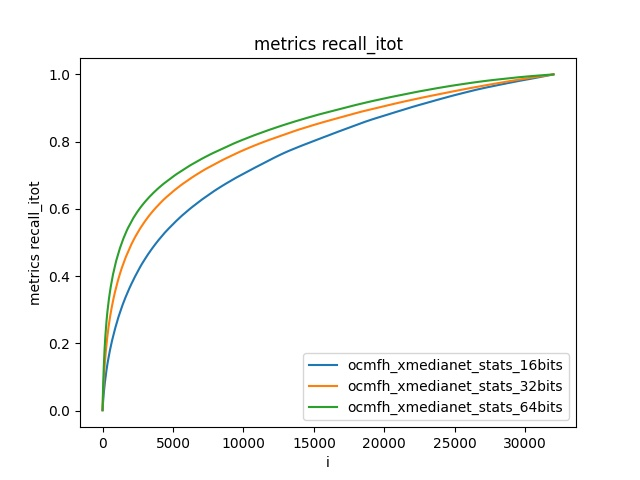
\includegraphics[width=\linewidth]{resultsImages/recall/metrics recall_itot_ocmfh_xmedia.jpeg}
                % \caption{Query type: countrange}
                % \label{fig:six_core_countrange}
                % \vspace{0.1ex}
                % \hspace{0.1ex}
            \end{minipage}
            \begin{minipage}[!h]{0.5\linewidth}
                \centering
                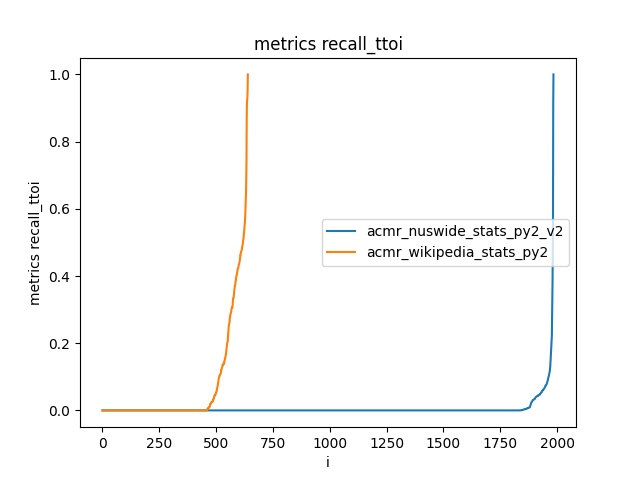
\includegraphics[width=\linewidth]{resultsImages/recall/metrics recall_ttoi_acmr_both.jpeg}
                % \caption{Query type: max}
                % \label{fig:six_core_max}
                % \vspace{0.1ex}
                % \hspace{0.1ex}
            \end{minipage}
            
            \begin{minipage}[!h]{0.5\linewidth}
                \centering
                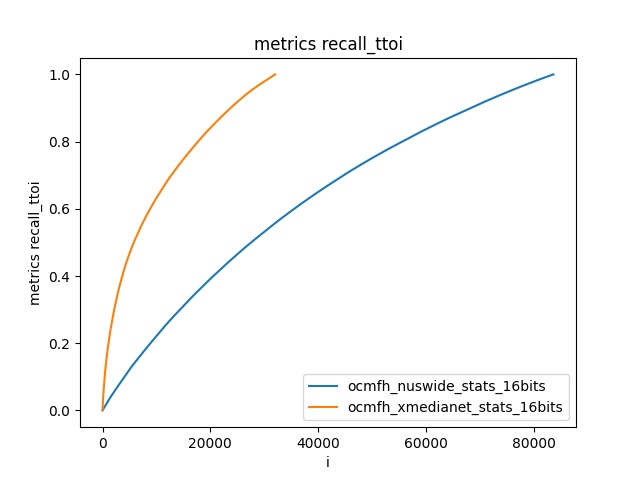
\includegraphics[width=\linewidth]{resultsImages/recall/metrics recall_ttoi_ocmfh_both.jpeg}
                % \caption{Query type: countrange}
                % \label{fig:six_core_countrange}
                % \vspace{0.1ex}
                % \hspace{0.1ex}
            \end{minipage}
            \begin{minipage}[!h]{0.5\linewidth}
                \centering
                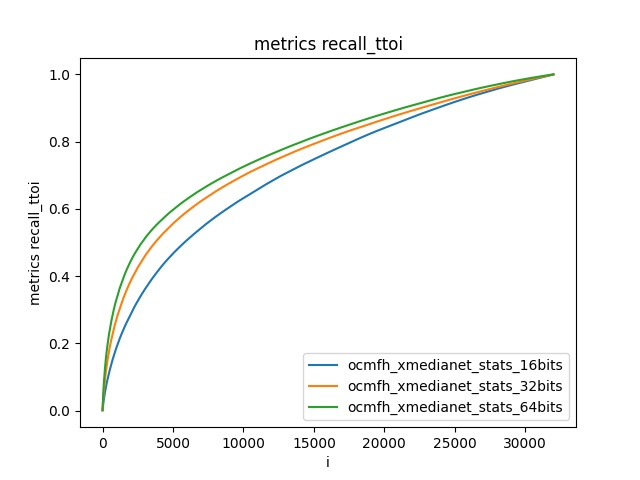
\includegraphics[width=\linewidth]{resultsImages/recall/metrics recall_ttoi_ocmfh_xmedia.jpeg}
                % \caption{Query type: max}
                % \label{fig:six_core_max}
                % \vspace{0.1ex}
                % \hspace{0.1ex}
            \end{minipage}
        \caption{Recall metric for ACMR and OCMFH on various datasets}
        \label{fig:}
        \end{figure}
        \FloatBarrier
    \subsection{Time}
    Following are the bar plots for training and execution time in seconds. Plots in the first row are the prediction and training time of OCMFH\cite{ocmfh} on two datasets(nuswide and xmedianet) with fixed bit vector length(16). Plot in the second row compares OCMFH\cite{ocmfh} and ACMR training time on nuswide dataset.
        \begin{figure}[H]
            \begin{minipage}[!h]{0.6\linewidth}
                \centering
                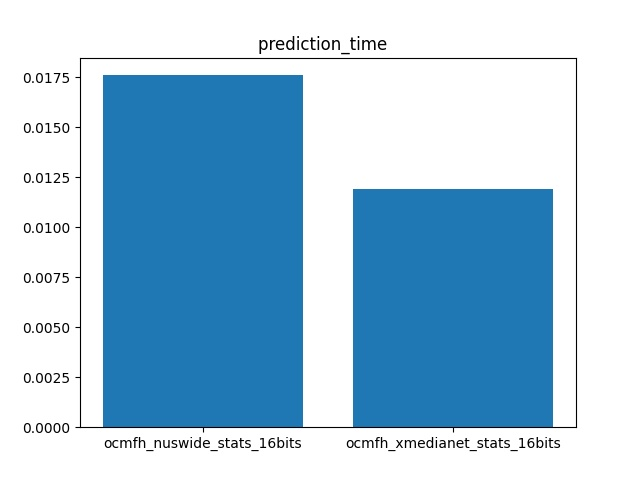
\includegraphics[width=\linewidth]{resultsImages/time/prediction_time_ocmfh_both.jpeg}
                % \caption{Inter comparison(NUS-WIDE)}
                % \label{fig:}
                \vspace{0.1ex}
                \hspace{0.1ex}
            \end{minipage}
            \begin{minipage}[!h]{0.6\linewidth}
                \centering
                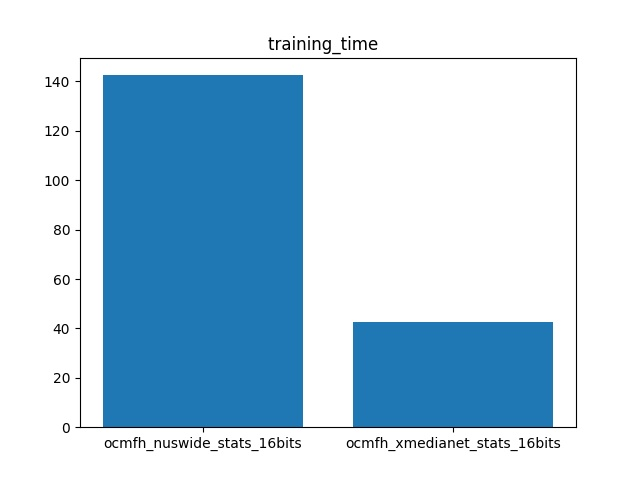
\includegraphics[width=\linewidth]{resultsImages/time/training_time_ocmfh_both.jpeg}
                % \caption{OCMFH chaning bits(Xmedianet)}
                % \label{fig:}
                \vspace{0.1ex}
                \hspace{1ex}
            \end{minipage}
            \begin{minipage}[!h]{0.8\linewidth}
                \centering
                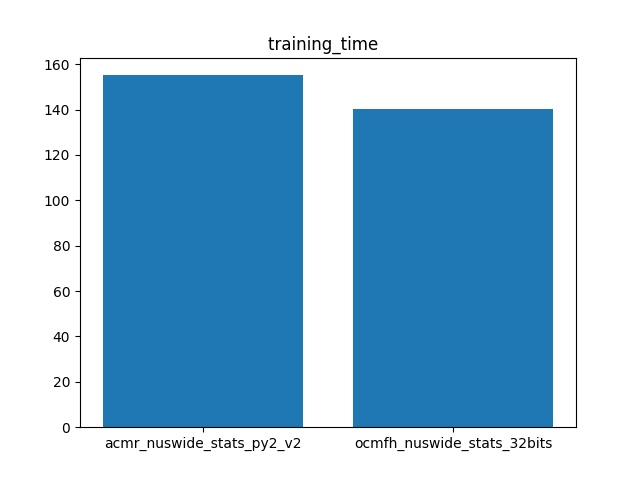
\includegraphics[width=\linewidth]{resultsImages/time/training_time _both_nuswide.jpeg}
                % \caption{OCMFH changing bits(NUS-WIDE)}
                % \label{fig:}
                \vspace{0.1ex}
                \hspace{0.1ex}
            \end{minipage}
            \caption{Training and prediction time for inter and intra method comparison on various datasets}
        \label{fig:}
        \end{figure}
        \FloatBarrier
    \subsection{Size}
    Following plots compares nuswide and xmedianet dataset statistics, e.g. number of classes and number of samples.
        \begin{figure}[H]
            \begin{minipage}[!h]{0.6\linewidth}
                \centering
                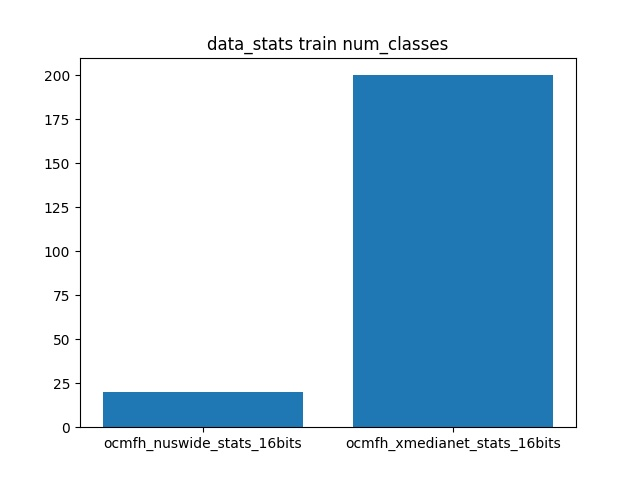
\includegraphics[width=\linewidth]{resultsImages/size/data_stats train num_classes.jpeg}
                % \caption{Inter comparison(NUS-WIDE)}
                % \label{fig:}
                \vspace{0.1ex}
                \hspace{0.1ex}
            \end{minipage}
            \begin{minipage}[!h]{0.6\linewidth}
                \centering
                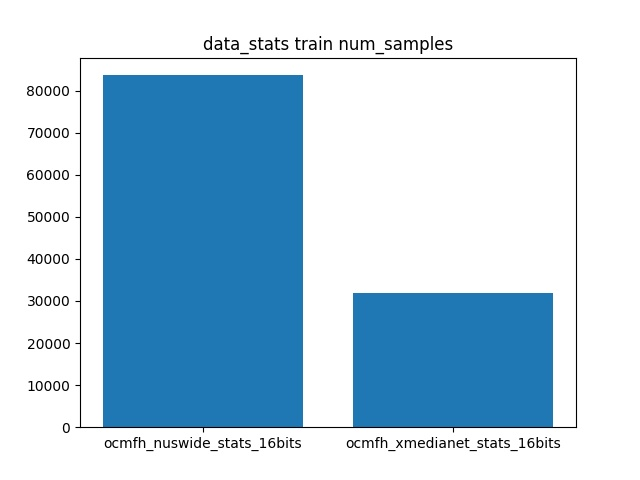
\includegraphics[width=\linewidth]{resultsImages/size/data_stats train num_samples.jpeg}
                % \caption{OCMFH chaning bits(Xmedianet)}
                % \label{fig:}
                \vspace{0.1ex}
                \hspace{1ex}
            \end{minipage}
            \caption{Dataset comparison in terms of \#classes and \#samples}
        \label{fig:}
        \end{figure}
        \FloatBarrier

\section{Comparison}
    \subsection{OCMFH}
In this section we compare the mAP score of OCMFH\cite{ocmfh} and ACMR\cite{acmr} between our implementation and scores mentioned in the original paper. \textbf{Note:} The comparison is not fair. In the original paper, the authors use vgg16 features for images. Whereas, we use bag of word features for images. The train and test split sizes are also different.

\begin{table}[!h]
    \centering
    \begin{tabular}{ | c | c | c | c | c |}
        \hline
         & Task & 32 bits & 64 bits & 128 bits
         \\ \hline
         OCMFH\cite{ocmfh} & itot & 0.8207 & 0.8455 & 0.8568
         \\ \hline
         OCMFH(our) & itot & 0.2269 & 0.2363 & 0.2329
         \\ \hline
         OCMFH\cite{ocmfh} & ttoi & 0.7675 & 0.7783 & 0.7863
         \\ \hline
         OCMFH(our) & ttoi & 0.2720 & 0.2869 & 0.2882
         \\ \hline
    \end{tabular}
    \caption{mAP on NUS-WIDE dataset}
    \label{table:}
\end{table}

\par Following can be the reasons behind such a large difference in the metric scores.
    \begin{itemize}
        \item They use only top-10 most frequent labels. We use top-20 most frequent labels.
        \item They use vgg16 features for image modality. We use simple bag-of-word features.
    \end{itemize}

\subsection{ACMR}
In the case of ACMR\cite{acmr}, we are exactly able to reproduce the results mentioned in the paper for wikipedia dataset. We have used the author's implementation of the code and have also taken the dataset provided with the code. This gives a fair comparison and proves that our framework is compatible with Real-valued retrieval algorithms. Information about the dataset is mentioned above in section 4.

\begin{table}[!h]
    \centering
    \begin{tabular}{ | c | c | c | c |}
        \hline
         & Img2Txt & Txt2Img
         \\ \hline
         ACMR\cite{ocmfh} & 0.489 & 0.619 
         \\ \hline
         ACMR(through framework) & 0.4671875 & 0.60625 
         \\ \hline

    \end{tabular}
    \caption{mAP on Wikipedia dataset}
    \label{table:}
\end{table}

If you see the paper, they have mentioned the wrong results. They have actually reversed the results for text to image and image to text in paper. If we run and verify the same from their code, we are able to generate the same results after running their code without framework and through our framework. 

\section{Links}
    \begin{itemize}
        \item \href{https://drive.google.com/file/d/1OYv7IK5OdDmBQ_pRXMugnqZzR_j7HOsu/view?usp=sharing}{Xmedianet dataset}
        , \href{https://lms.comp.nus.edu.sg/wp-content/uploads/2019/research/nuswide/NUS-WIDE.html}{NUS-WIDE dataset}
        \item \href{https://github.com/shivangibithel/ACMR_demo/tree/master/data}{Wiki}
        , \href{https://github.com/shivangibithel/ACMR_demo/tree/master/data}{NUS-WIDE 10K}
        \item \href{https://github.com/Prabhat1808/Multimodal-IR-Ablation}{Source Code}
        \item \href{https://www.cse.iitd.ac.in/~cs5170407/}{Framework Documentation}
    \end{itemize}


\bibliographystyle{alpha}
\bibliography{report}
\end{document}
























% bit length comparison in ocmfh